\section{Experiments}
\label{sec:experiments}

LLM-based experiments use the local model of \cref{sec:system}. For the benchmark comparisons, local
(LLM and simulated-annealing) conditions are repeated three times and reported as a mean with range;
real hardware is run once per condition. The later functional integration checks in
\cref{sec:integrationchecks} are reported separately from these performance experiments.

\subsection{Twelve problem categories, end to end}
\label{sec:suite}
For each of 12 categories (scheduling, routing, location, assignment, knapsack, portfolio, graph partitioning,
set cover, clustering, network design, resource allocation, feature selection) we wrote one realistic sentence and
ran the full pipeline three times, answering every clarification question with the agent's own suggested default.
These runs use the model's synthetic data generator, so they test the pipeline, not real-data handling.

All 36 clarifications converged and were confirmed (median 5.6 minutes per pipeline). All 36 models passed
validation and 35 produced a validated figure. Two of our own checks were initially wrong and are reported as
such: a too-strict ``solvable by sorting'' test rejected every assignment, set-cover and network-design model
(constraints that overlap are not sortable), and the figure step was skipped whenever brute force was impossible.
Both were fixed and the affected categories rerun.

\Cref{tab:suite} reports one solve per category on the GPU annealer and on simulated annealing with default
parameters. Where an exact optimum is known, the GPU annealer reached it in 7 of 9 categories. It found no feasible
portfolio, and network design, whose connectivity requirement is hard to express as a QUBO, remained far from
optimal on both solvers.

\begin{table}[t]
\centering
\caption{One solve per category of the first valid model, small synthetic instances (12 to 144 variables).
Gap to the exact optimum where known; otherwise the objective (lower is better unless noted).}
\label{tab:suite}
\small
\begin{tabular}{@{}lrll@{}}
\toprule
Category & Vars & GPU annealer & SA (default) \\
\midrule
Location & 132 & optimal & optimal \\
Assignment & 144 & optimal & +17.0\% \\
Knapsack & 12 & optimal & +5.4\% \\
Graph (max-cut) & 12 & optimal & optimal \\
Set cover & 12 & optimal (1 sensor) & 5 sensors \\
Resource allocation & 52 & optimal & no feasible solution \\
Feature selection & 12 & optimal & optimal \\
Portfolio & 12 & no feasible solution & optimal \\
Network design & 66 & feasible 0.5\%, $8.6\times$ optimum & no feasible solution \\
Routing & 144 & 475 & 557 \\
Clustering & 36 & 33{,}801 & 34{,}257 \\
Scheduling & 112 & tie & tie \\
\bottomrule
\end{tabular}
\end{table}

\subsection{Scaling of a GPU annealer on routing}
The routing model the local LLM wrote for a single-vehicle tour uses position encoding ($n^2$ variables for $n$
stops). We solved it once per size on the GPU annealer with default parameters (10-second jobs) and compared with
the exact optimum (Held--Karp, $n\le 13$) or a 2-opt reference with 20 restarts. Every returned tour was feasible
up to 3{,}600 variables. Quality was exact up to 10 stops and matched the 2-opt reference up to 30 stops (900
variables), then degraded: $+12.4\%$ at 40, $+27.2\%$ at 50 and $+43.5\%$ at 60 stops. Simulated annealing with
default parameters degraded much earlier ($+6.5\%$ at 8 stops, $+164\%$ at 30). These large instances are where
tuning can matter. \pending{tuning loop on the GPU annealer at 40--60 stops}

\subsection{LLM-driven tuning versus baselines}
\label{sec:tuningcomparison}
On simulated annealing, we compared seven tuning policies at equal solver budgets on 80 paired runs each
(knapsack and select-$k$ instances of 40 to 80 items, 10 seeds). The three agent variants reached a lower mean gap
(0.073--0.078) than default parameters (0.084), rule-based tuning (0.088), random search (0.090) and Optuna
(0.092); all agent-versus-baseline differences are significant (paired Wilcoxon, $p\le 0.0064$). The improvement is
small, and default parameters found the optimum more often (38/80 versus 25--35/80). Splitting the tuning agent
into diagnoser and refiner roles did not help ($p=0.10$), nor did retrieval of tuning knowledge ($p=0.17$). We
read this as a consequence of easy instances on which defaults already do well, and repeat the comparison on hard
instances and hardware. \pending{hard instances (large routing, QOBLIB) on the GPU annealer and Fujitsu DA}

\subsection{Penalty tuning is a secondary step}
\label{sec:penaltysummary}
Penalty tuning can improve feasibility or quality, but it cannot repair wrong data or a missing constraint.
On eight synthetic knapsack and select-$k$ instances with local SA (640 runs, ten seeds), default weights had the
lowest mean gap (0.093); every penalty-search policy (TPE, grid, cross-entropy, sequential) was worse (Holm-adjusted
$p=0.03$). The defaults sit just above a feasibility floor, and the search ranges reach 16 times higher, so with six
calls the searches mostly sampled over-penalised settings. On the GPU annealer the picture differs: for the frozen
red-wine model the default weights left a mean gap of 0.550, penalty TPE reduced it to 0.074 and the tuning agent
to 0.000 (three submissions each), while on two other models the defaults already reached the exact optimum. The
UI therefore starts with the default policy and exposes tuning as an alternative; data and model faults have
separate upstream recovery paths. This default selection is not an automatic policy-switching experiment. Reproduction settings and ancillary
solver checks are summarized in \cref{app:details}.

\subsection{Frozen-model backend comparison}
\label{sec:additionalexperiments}
\label{sec:dwavehybrid}
The red-wine, 60-item knapsack and 80-item conflict-selection models were frozen before comparing defaults,
TPE penalty search and an LLM tuning agent. SA and CGA produced feasible solutions in all 54 conditions;
Leap Hybrid BQM produced feasible solutions in all 27 conditions, using 72 submissions with an explicit
ten-second limit per call. Table~\ref{tab:backendkeyresults} reports selected mean gaps to exact references.

\begin{table}[t]
\centering\small
\caption{Mean gaps on frozen models, three repetitions per policy. Budgets differ across backends;
these results do not establish hardware superiority.}
\label{tab:backendkeyresults}
\begin{tabular}{@{}llrrr@{}}
\toprule
Backend & Model & Default & TPE search & LLM tuning \\
\midrule
CGA & Red wine & 0.5495 & 0.0740 & 0.0000 \\
Leap Hybrid & Red wine & 0.0000 & 0.0000 & 0.0000 \\
Leap Hybrid & Knapsack (60 items) & 0.1060 & 0.1164 & 0.1149 \\
Leap Hybrid & Selection (80 items) & 0.0000 & 0.0141 & 0.0016 \\
\bottomrule
\end{tabular}
\end{table}

CGA defaults reached the reference on the other two models. The Hybrid results are service-level results,
not direct-QPU sampling. A Fujitsu DA submission was rejected at the account's monthly usage limit;
no successful DA result is claimed. These fixed-model comparisons evaluate solver behaviour, not the full
LLM acquisition and modelling workflow.

\subsection{Mechanisms for a small local model}
\label{sec:mechanisms}
\begin{itemize}
  \item \emph{Constraint families.} On a 12-nurse, 28-day scheduling model (1{,}680 variables, 3{,}324
        constraints) the tuning prompts listed every constraint and overflowed the 64k-token context. Showing the
        10 constraint families instead reduced the configurator and diagnoser prompts from about 53k--54k to
        2k--3k tokens; decisions taken for a family are expanded to its members by code.
  \item \emph{Task splitting.} Asking the Modeling Agent for the model and its figure in one answer exhausted its
        reasoning budget repeatedly; with the figure moved to a separate short task, autonomous modelling of an
        EV-charger siting problem succeeded in 2 of 3 runs (about 6 minutes each), each with a figure.
  \item \emph{Repair, not rewrite.} Retries that show the previous module avoided regressions in which an almost
        correct model (one indexing error) was replaced by a worse one.
  \item \emph{Reasoning budget.} With a per-call cap and a single retry without reasoning, empty answers of the
        Coder fell from 7 of 240 calls (2.9\%) to 5 of 521 (1.0\%).
\end{itemize}

\subsection{Real data}
\label{sec:realdata}
As a first check of the preprocessing toolkit on real public data, we reproduced Taipei's per-village population
from the city's published table (63{,}315 rows; ROC years, stacked months, rows split by gender, city and
district totals mixed with villages) and joined it with the official village boundary layer (TWD97 coordinates).
The cleaned total, 2{,}418{,}872, equals the city total published in the same table; 455 of 456 villages matched
by name and the last one only after allowing a variant character (the two official tables spell one village name with different characters).
An early version of one tool kept the city-total row as a village and doubled the population; the provenance
record, which reports row counts and totals, is what exposed it.


\paragraph{Specified-source pilots.}
A UCI red-wine case\footnote{\url{https://archive.ics.uci.edu/dataset/186/wine+quality}} used all 1,599 records;
the local LLM generated model and Adapter code, and a five-feature selection matched the objective
0.7497088247 after four SA calls, checked against all 2,048 assignments. A recovered wholesale-customer
case\footnote{\url{https://archive.ics.uci.edu/dataset/292/wholesale+customers}} formed three groups of eight
from 24 sampled records, obtaining 856.8319 versus a feasible baseline of 1021.7818 (16.1\% lower).
A recovered karate-club case\footnote{\url{https://websites.umich.edu/~mejn/netdata/}} delivered two groups
of 17 with 17 cut edges from the conventional baseline, because annealing returned 22 cut edges.
These pilots used manually specified inputs or case-specific checks, and some reused generated artifacts.
They establish narrower integration capabilities than autonomous acquisition from an unrestricted request.

\subsection{Autonomous real-data acceptance: protocol}
\label{sec:autonomousprotocol}
Every run starts without a saved model, instance or LLM cache, and every arm, including the direct-LLM baseline,
must search for and download its own data. The system receives the original request and fixed user answers that
contain settings only (counts, areas, distance definitions), never field names or formulas. The development set
has five problem families, each in a small and a large version, chosen so that problem structure, data
difficulty, size, country and language vary independently (\cref{tab:devcases}).

\begin{table}[t]\centering\small
\caption{Development cases. Truth is computed from official raw files by separate code; the London and Berlin
references are exact MILP optima.}
\label{tab:devcases}
\begin{tabular}{@{}p{2.6cm}p{3.05cm}p{2.4cm}p{2.45cm}p{3.85cm}@{}}\toprule
Family & Structure & Small & Large & Main data difficulty \\\midrule
Taipei EV chargers & max coverage, count once & 53 villages, $k=3$ & 456 villages, $k=5$ & two sources, TWD97, totals, yearly files \\
YouBike tour & routing & 18 stations & 38 stations & live feed, radius filter \\
Taipei AED teams & balanced partition & 48 places, 3 teams & 200 places, 4 teams & duplicates per place, category filter \\
London ambulance & $p$-median & 27 MSOAs, $p=3$ & 256 LSOAs, $p=8$ & British grid, census + centroids \\
Berlin playgrounds & new coverage (250\,m) & 36 candidates, $k=3$ & 145 candidates, $k=8$ & three sources, WFS, German, point in polygon \\
\bottomrule\end{tabular}\end{table}

\paragraph{Mechanism comparisons.}
\Cref{fig:acceptancedesign} shows which mechanisms each arm enables and how runs are judged.
\begin{enumerate}
  \item \emph{Direct LLM}: ordinary web search and download, then one LLM-written module for preprocessing and
        modelling, with Python-error feedback only.
  \item \emph{Structured workflow}: clarification, structured schema, acquisition with platform connectors,
        toolkit-enforced adaptation and data contracts, without independent checkers or cross-stage repair.
  \item \emph{Workflow with checkers}: the pipeline plus the Data and Requirement Checkers (detection only).
  \item \emph{Complete workflow}: checkers plus bounded cross-stage repair.
  \item \emph{Workflow with retrieval}: the complete workflow plus retrieval of modelling patterns.
  \item \emph{Without clarification web lookup}: the complete workflow with the Clarifier's web lookup disabled;
        data acquisition still searches the web.
\end{enumerate}
The budget allows three clarification rounds, four modelling attempts, two acquisition search rounds, at most
four downloads, three solver calls on CGA with the default policy, one pre-solve model repair and two workflow
repairs. The direct downloader has its own three-file cap and uses the same network settings as the pipeline.
Comparing the direct LLM with the structured workflow compares complete configurations; it does not isolate the
causal effect of multiple agents. Adjacent pipeline arms estimate the effects of checking and repair under these
budgets. Each run records time, tokens, solver calls, failed stage, repair history, delivery source and which
truth was used. Automated confirmations and fixed answers are fixtures, not measurements of user effort.

\begin{figure}[tbp]
\centering
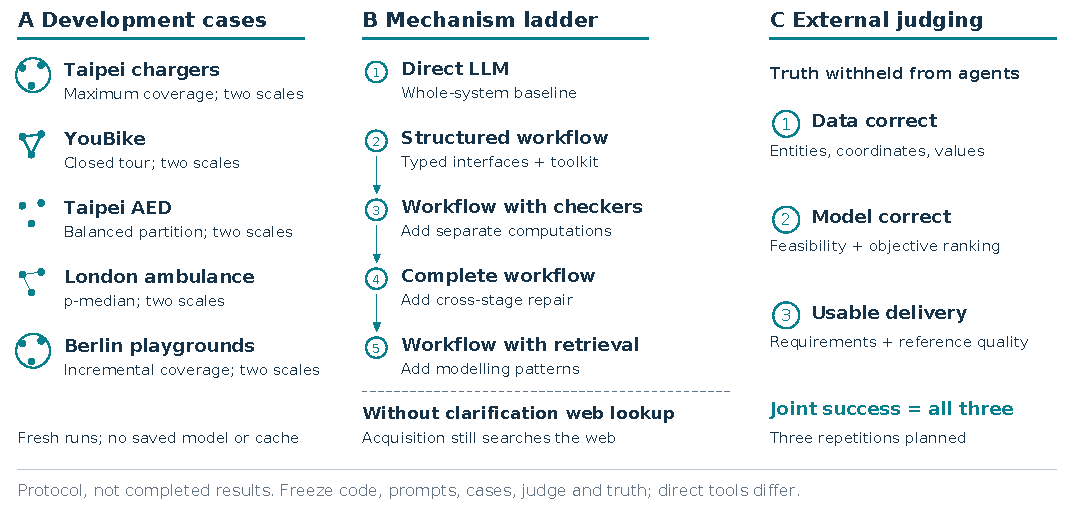
\includegraphics[width=\linewidth]{figures/skill/acceptance-design.pdf}
\caption{Design of the autonomous acceptance comparison, not completed experimental results.
Five development families each have two scales. The ladder identifies the added mechanism in each pipeline configuration; the separate web-lookup arm retains data acquisition.
The direct baseline uses different tools and download limits, so its comparison with the pipeline cannot
isolate agent count. Joint success requires all three acceptance outcomes.}
\label{fig:acceptancedesign}
\end{figure}


\paragraph{External acceptance criteria.}
A deterministic judge reads truth that is never supplied to the runtime agents. \emph{Data:} the instance's
entities must map one-to-one to real entities, by identifier or name first and by coordinates (within a
case-specific tolerance) only for what remains; name-matched entities must still have coordinates near their
own entity and no two entities may share coordinates; measured values must match entity by entity and totals
must equal the official figures. \emph{Model:} with the decision variables fixed to 30 sampled decisions that
satisfy the original request (for selection cases, half of them clustered so that service areas overlap) and
helper variables optimized by MILP, the model must accept every sample and rank them like the independent
metric (Spearman $\geq 0.9$); decisions that break the request must be rejected. \emph{Delivery:} the delivered
solution must satisfy the original request and stay within 10\% of a reference computed on the raw data
(greedy selection, nearest neighbour with 2-opt, greedy grouping with swaps, or the exact optimum). Solutions
from the annealer and from the conventional baseline both count, and are reported separately. A model the judge
cannot read, or cannot compare because the data are wrong, is ``unverifiable'' and counts as incorrect in the
primary analysis. For live feeds, the truth is recomputed from the very official file the run downloaded; runs
that used another source are judged against a pre-downloaded official snapshot and flagged. The judge never
raises: unexpected output becomes a failed or unverifiable gate. Self-tests confirm that correct synthetic
outputs pass and deliberately broken ones fail (dropped entities, copied coordinates, unconverted projected
coordinates, a relaxed cardinality bound, a scattered grouping, a poor tour).

\paragraph{Freezing, preregistration and held-out cases.}
Code, prompts, the modelling-pattern library, solver configuration, case definitions, judge and truth are hashed
before a batch; any change requires a new batch tag. A preflight script must pass before a batch starts (tests,
judge self-tests, a truth and a judge for every case, LLM server, solver reachability, hardware budget, no other
experiment running). Hypotheses, metrics, the treatment of unverifiable models and the rerun rule (only
infrastructure failures) are fixed in advance. The development cases, the modelling-pattern library and the judge
were revised after observing development runs; generalization is therefore assessed on held-out cases defined and
run only after the code is frozen again.

\paragraph{Development observations.}
Development runs used changing code and are not a frozen comparison; they are reported for the failure modes they
revealed, not as rates. Mechanisms behaved as designed in several instances: the toolkit's join flags rejected
a village-name join that would have merged homonymous villages and reduced 456 villages to 32; a schema mismatch
found during data preparation (non-unique village names used as identifiers) was routed back to the Modeling
Agent, repaired, and the run delivered an accepted solution; the data double-check exposed an AED instance with
320 rows instead of 48 places and a fabricated extra station. The LLM-written checkers were also wrong several
times: a Data Checker summed category rows twice, a Requirement Checker computed great-circle distances without
converting degrees to radians, and another invented a fixed start station. The last one made the controller
discard an annealer tour shorter than the reference in favour of a weaker baseline, which motivated two rules:
a late Checker objection does not trigger a repair when no solver call remains to re-solve, and a repaired
version without a solution falls back to the earlier version's annealer result. Other recurring failures were
a modelling-technique (subtour elimination) recorded as a user requirement, an edge-based tour model without a
single-tour guarantee, crowd-sourced points used instead of a named official feed, and report spreadsheets
mistaken for record tables; each led to a problem-independent rule or check described in \cref{sec:system}.
We report no aggregate autonomous success rate or mechanism effect yet.
